%; whizzy paragraph -pdf xpdf -latex ./whizzypdfptex.sh
%; whizzy-paragraph "^\\\\begin{frame}"
% latex beamer presentation.
% platex, latex-beamer でコンパイルすることを想定。 

%     Tokyo Debian Meeting resources
%     Copyright (C) 2009 Junichi Uekawa
%     Copyright (C) 2009 Nobuhiro Iwamatsu

%     This program is free software; you can redistribute it and/or modify
%     it under the terms of the GNU General Public License as published by
%     the Free Software Foundation; either version 2 of the License, or
%     (at your option) any later version.

%     This program is distributed in the hope that it will be useful,
%     but WITHOUT ANY WARRANTY; without even the implied warreanty of
%     MERCHANTABILITY or FITNESS FOR A PARTICULAR PURPOSE.  See the
%     GNU General Public License for more details.

%     You should have received a copy of the GNU General Public License
%     along with this program; if not, write to the Free Software
%     Foundation, Inc., 51 Franklin St, Fifth Floor, Boston, MA  02110-1301 USA

\documentclass[cjk,dvipdfmx,12pt]{beamer}
\usetheme{Tokyo}
\usepackage{monthlypresentation}

%  preview (shell-command (concat "evince " (replace-regexp-in-string "tex$" "pdf"(buffer-file-name)) "&")) 
%  presentation (shell-command (concat "xpdf -fullscreen " (replace-regexp-in-string "tex$" "pdf"(buffer-file-name)) "&"))
%  presentation (shell-command (concat "evince " (replace-regexp-in-string "tex$" "pdf"(buffer-file-name)) "&"))

%http://www.naney.org/diki/dk/hyperref.html
%日本語EUC系環境の時
\AtBeginDvi{\special{pdf:tounicode EUC-UCS2}}
%シフトJIS系環境の時
%\AtBeginDvi{\special{pdf:tounicode 90ms-RKSJ-UCS2}}

\title{東京エリアDebian勉強会}
\subtitle{第75回 2011年5月度}
\author{岩松 信洋 iwamatsu@debian.org\\IRC nick: iwamatsu}
\date{2011年5月21日}
\logo{
\includegraphics[width=8cm]{image200607/openlogo-light.eps}}

\begin{document}

\frame{\titlepage{}}

\section{}
\begin{frame}
 \frametitle{Agenda}
\begin{minipage}[t]{0.45\hsize}
  \begin{itemize}
  \item 注意事項
	\begin{itemize}
	 \item 飲酒禁止
	 \item 宗教禁止
	 \item 営利活動禁止
	\end{itemize}
   \item 最近あったDebian関連のイベント報告
	\begin{itemize}
	 \item 第75回 東京エリア Debian勉強会
         \item 第 46 回関西 Debian 勉強会@OSC2011 Kobe
	\end{itemize}
 \end{itemize}
\end{minipage} 
\begin{minipage}[t]{0.45\hsize}
 \begin{itemize}
  \item Apache2 のモジュールをつくってみた
  \item Debian on NiftyCloud
  \item Debian/m68k 開発
  \item 月刊PPC64ポーティング
 \end{itemize}
\end{minipage}
\end{frame}

\begin{frame}
 \frametitle{前回}
\begin{minipage}[t]{0.45\hsize}
  \begin{itemize}
  \item 注意事項
	\begin{itemize}
	 \item 飲食禁止
	 \item 宗教禁止
	 \item 営利活動禁止
	\end{itemize}
  \end{itemize}
\end{minipage}
\begin{minipage}[t]{0.45\hsize}
\begin{itemize}
  \item 最近あったDebian関連のイベント報告
 \begin{itemize}
  \item 会長就任挨拶
  \item backports.debian.orgの話
  \item initramfs-toolsの話
  \item 月刊PPC64ポーティング
  \item 僕がDD目指すの手伝ってください
 \end{itemize}
 \end{itemize}
\end{minipage}
\end{frame}


\emtext{イベント報告}

\emtext{DWN quiz}

\section{DWN quiz}
\begin{frame}{Debian 常識クイズ}

Debian の常識、もちろん知ってますよね?
知らないなんて恥ずかしくて、知らないとは言えないあんなことやこんなこと、
みんなで確認してみましょう。

今回の出題範囲は\url{debian-devel-announce@lists.debian.org} に投稿された
内容とDebian Project Newsからです。

\end{frame}

\subsection{問題}
%; whizzy-master ../debianmeetingresume201101.tex
% $B0J>e$N@_Dj$r$7$F$$$k$?$a!"$3$N%U%!%$%k$G(B M-x whizzytex $B$9$k$H!"(Bwhizzytex$B$,MxMQ$G$-$^$9!#(B
%
% $B$A$J$_$K!"%/%$%:$OJL%V%i%s%A$G:n@.$7!"$N$A$K%^!<%8$7$^$9!#5U$K%^!<%8$7(B
% $B$J$$$h$&$K$7$^$7$g$&!#(B
% (shell-command "git checkout quiz-prepare")

\santaku
{HPPA $B$H(B alpha $B$N0\E>@h$O$I$3$G$7$g$&$+!)(B}
{buildd.debian.or.jp}
{buildd.debian-ports.org}
{www.buildd.net}
{B}
{}

\santaku
{linux$B%+!<%M%k(B 2.6.39$B$,(BDebian$B$KF~$k$3$H$K$h$C$F5/$-$kJQ99$O!)(B}
{i386-bigmem$B$,(Bi386-pae$B$K$J$C$?(B}
{amd64$B$,(Bi386$B$K$J$C$?(B}
{i386$B$O(Bamd64$B$N%^%k%A%P%$%J%j$K$J$C$?(B}
{A}
{}

\santaku
{Qt3$B%Q%C%1!<%8$,:o=|$5$l$J$$M}M3$O!)(B}
{Qt3$B%f!<%6$K$h$k0%4j$N$?$a(B}
{LSB 4.1$B$,(BQt3$B$rI,MW$H$7$F$$$k$?$a(B}
{$B:o=|$N;EJ}$,$o$+$i$J$$(B}
{B}
{}

\santaku
{Debian$B$N%5!<%P$KDI2C$5$l$?5!G=$O!)(B}
{$B%m%0%$%s$7$F$$$k%f!<%6$r(BIRC$B$KN.$95!G=(B}
{RFC1149 $B$N<BAu(B}
{DNSSEC}
{C}
{}


\emtext{prework}

{\footnotesize
 %; whizzy-master ../debianmeetingresume201101.tex
% $B0J>e$N@_Dj$r$7$F$$$k$?$a!"$3$N%U%!%$%k$G(B M-x whizzytex $B$9$k$H!"(Bwhizzytex$B$,MxMQ$G$-$^$9!#(B



\begin{prework}{ $B%-%?%O%i(B }

Debian$B8BDj$@$H;W$$$D$+$J$$!&!&!&!#(B
($B$*Bj$N0U?^$rFI$_0c$($F$$$k$N$+$b(B)
apt-get$B$r(Bhttp$B$G<B9T$9$k$H%&%'%V%5!<%S%9$H8@$($k(B?
\end{prework}

\begin{prework}{ MATOHARA }

Debian$B;H$$$H$7$F%&%'%V%5!<%S%9$K4|BT$9$k$3$H!%(B
$B:G6a$O>/$J$/$J$j$^$7$?$,!$(BIE $BI,?\$N%5!<%S%9Ey$N4D6-0MB8$N%5!<%S%9$r$d$a(B
 $B$FM_$7$$$G$9!%(B
$B:G6a$@$H(BSilverlight $BI,?\$N%5!<%S%9$G(BMoonlight $B$GF0$-$=$&$GF0$+$J$$$H$$$C(B
 $B$?$3$H$,$"$j$^$7$?!%(B
\url{http://live6.channel.ne.jp/world_ipv6/}
\end{prework}

\begin{prework}{ taitioooo }

$B>pJs$KBP$9$k2]6b$,$J$/$J$k$3$H!#(B

\end{prework}

\begin{prework}{ $BLnEg!!5.1Q(B }

\begin{itemize}
\item jslinux$B$H$$$&6/NO$J%(%_%e%l!<%?$b=P$?$N$G!"%V%i%&%6$GF0$/(BDebian
 experimental$B4D6-$H$+%V%i%&%6$GF0$/(BGnome$B$N$*;n$74D6-$H$+$rDs6!$9$k%&%'%V(B
 $B%5!<%S%9$H$+AGE($+$b!#(B
$B$3$b$-$C$H%&%'%V%5!<%S%9!*!J$J$s$+6u5$FI$a$F$J$$2sEz$J5$$b$9$k$1$I(B...)

\item USB$B$K=q$-9~$a$P(Bdebian$B4D6-$,$=$N$^$^%V!<%H$G$-$k$h$&$J%$%a!<%8$r$D$/$C$F(B
 $B$/$l$k%&%'%V%5!<%S%9$,NI$5$=$&$J5$$b(B...$BNc$($P!"%Q%C%1!<%80lMw$K%A%'%C%/(B
 $BF~$l$F!"(Bsid$B$H$+$K%A%'%C%/F~$l$k$H!"(BUSB$B%a%b%j$K$=$N$^$^=q$-9~$a$P$=$N;E(B
 $BMM$G(Bdebian sid$B$,%V!<%H$G$-$k$h$&$J%+%9%?%`%$%a!<%8$r:n$C$F$/$l$k$H$+!#(B

\item $B%A%'%C%/%\%C%/%9$H%;%l%/%?$@$1$G!"(Bpreceed$B%U%!%$%k@8@.$7$F$/$l$k%&%'%V%5!<(B
 $B%S%9$b$$$$$+$b(B...$BBgNL$N%$%s%9%H!<%k;~$H$+$h$5$=$&!#(B
$B!J$b$&8@$$$?$$J|Bj$G$9$M(B...)
\end{itemize}











\end{prework}

\begin{prework}{ $B4d>>(B $B?.MN(B }
\begin{itemize}
\item $BA4@$3&$N(BWeb$B%5!<%P$rDs6!$9$k(BOS$B$,(BDebian$B$K$J$k$3$H!#(B
\item $BJ,;6%3%s%Q%$%k%5!<%P$H$+M_$7$$!#(B
\end{itemize}


\end{prework}

\begin{prework}{ $BF|HfLn(B $B7<(B }

Web$B%5!<%S%9$b$G$-$l$P5!3#=hM}$7$d$9$$$b$N$,NI$$!#(B
$B$"$H!"%/%i%&%I>e$G$N(BAPI$B$rDs6!$7$F$$$k$h$&$J%5!<%S%9$K!"4X?t7?8@8l$KBP$9(B
 $B$k%5%]!<%H$,A}$($F$[$7$$!#(B

\end{prework}

\begin{prework}{ dictoss($B?yK\!!E5=<(B) }

CPU$B$H$"$k(Bdeb$B%Q%C%1!<%8$rA*Br$9$k$H!"$=$N(BCPU$B8~$1$K:GBg8B$N:GE,2=$7$?%Q%C(B
 $B%1!<%8$H0MB8$9$k%Q%C%1!<%8$r:F%S%k%I$7$F$/$l$k%5!<%S%9!#(B
\end{prework}

\begin{prework}{ kazken3 }

$BK]Lu$r$?$^$K$7$F$$$k$N$G!"%G%#%9%H%j%S%e!<%7%g%s4V2#$I$*$7$G$NK]Lu4XO">p(B
 $BJs$rDs6!$9$k%5%$%H$,$"$l$P$$$$$J$H;W$&$3$H$,$"$j$^$9!#(B

$B!t2]Bj$H$O>/$7%:%l$F$$$k$+$bCN$l$^$;$s$,!"(B
$B!t8D?M8~$1$N%&%'%V%5!<%S%9$K$O?)=}5$L#$H$$$&$H$3$m$b$"$k$N$G!#(B


\end{prework}

\begin{prework}{ $B$^$($@$3$&$X$$(B }

Debian$B%7%9%F%`$G:n$C$?4D6-$H$NAj8_8_49@-!#(B
$BNc$($P!":G6a(BGAE/Python$B$r$h$/;H$&$N$G!":n$C$?%7%9%F%`$r(B
 GAE/Python <-> $B"*(BDebian$B%7%9%F%`$N$I$A$i$G$b(B($B$[$H$s$IJQ99$J$7$G(B)$BF0$+$;$k$H(B
 $BJXMx$G$9$M!#(B
$B$9$0;O$a$k$N$K%/%i%&%I%5!<%S%9$rMxMQ$7$F:n$C$?$1$I>-Mh$O(BDebian$B$GF0$+$7$?(B
 $B$$!"5U$K:#$O@/<#E*$JM}M3$G30$K=P$;$J$$(BDebian$B%7%9%F%`$r>-Mh$O<+J,$N4IM}(B
 $B$+$i30$l$k$N$G<jN%$l$r$h$/$9$k$?$a$K%/%i%&%I%5!<%S%9$K4JC1$K0\9T$G$-$k!"(B
 $B$J$I!#(B
\end{prework}

\begin{prework}{ yamamoto }

$B$=$&$G$9$M!#(B
$B:#$N=jF3F~$r8!F$$7$F$$$k$N$O!"%Q!<%=%J%k%9%H%l!<%8%5!<%S%9$0$i$$$G$9$+$M!#(B
$B$"$i$f$k=j$G<+J,$N%G!<%?$,<+J,$G6&M-$G$-$l$P!"$=$l$G==J,$J46$8$G$9!#(B
\end{prework}

}

\emtext{Apache2 のモジュールをつくってみた}

\begin{frame}{Apache2 モジュール入門}
\begin{itemize}
 \item apache httpd で動くモジュール
 \item C言語で実装
 \item Debianの流儀
\end{itemize} 
\end{frame}

\begin{frame}[containsverbatim]{apxs2: テンプレ作成}
\begin{commandline}
$ apxs2 -g -n dancerqps
$ cd dancerqps
$ ls 
$ ls
Makefile  mod_dancerqps.c  modules.mk
\end{commandline}
\end{frame}

\begin{frame}{コードを書く}
 
適当にフックを記述

\end{frame}

\begin{frame}[containsverbatim]{apxs: インストール}

コンパイルしてインストール
 \begin{commandline}
 $ sudo apxs2 -c -i mod_dancerqps.c
 \end{commandline}
\end{frame}

\begin{frame}{実行}
 4種類方法があります。
\begin{itemize}
 \item Debian way 1 a2enmod
 \item Debian way 2 手動で設定
 \item Apache を適当なhttpd.confで起動
 \item Apache を自前でインストールしなおす 
\end{itemize}
\end{frame}

\begin{frame}[containsverbatim]{適当なhttpd.conf}
 \begin{commandline}
Listen 8080

LockFile /home/test/tmp/apache.1.lock
PidFile /home/test/tmp/apache.1.pid

# log configuration.
LogFormat "%h %l %u %t \"%r\" %>s %b" common
CustomLog "/home/test/log/access_log" common
ErrorLog "/home/test/log/error_log"

# Order, Allow.
LoadModule authz_host_module /usr/lib/apache2/modules/mod_authz_host.so
# map from / -> /index.html
LoadModule dir_module /usr/lib/apache2/modules/mod_dir.so
DirectoryIndex index.html index.cgi index.pl index.php index.xhtml index.htm
# .html -> content-type: text/html
LoadModule mime_module /usr/lib/apache2/modules/mod_mime.so
TypesConfig /etc/mime.types

# Document root
DocumentRoot "/home/test/hoge"
<Directory "/home/test/hoge">
    Options Indexes FollowSymLinks

    AllowOverride None

    Order allow,deny
    Allow from all

</Directory>

# Load my custom filter.
LoadModule dancerqps_module /usr/lib/apache2/modules/mod_dancerqps.so
SetOutputFilter DANCERQPS
 \end{commandline}
\end{frame}

\begin{frame}[containsverbatim]{apache 実行}
\begin{commandline}
APACHE_RUN_USER=dancer \
 APACHE_RUN_GROUP=dancer \
 /usr/sbin/apache2 -f $(readlink -f ./httpd.conf) -k restart 
\end{commandline} 
\end{frame}

\begin{frame}[containsverbatim]{apachebench 使ってみる}
 \begin{commandline}
$ /usr/sbin/ab -c 100 -n 100 http://localhost:8080/
 \end{commandline}
\end{frame}

\begin{frame}[containsverbatim]{apache 実行}
\begin{commandline}
$ /usr/sbin/ab -c 100 -n 100 http://localhost:8080/ 
This is ApacheBench, Version 2.3 <$Revision: 655654 $>
Copyright 1996 Adam Twiss, Zeus Technology Ltd, http://www.zeustech.net/
Licensed to The Apache Software Foundation, http://www.apache.org/

Benchmarking localhost (be patient).....done


Server Software:        Apache/2.2.9
Server Hostname:        localhost
Server Port:            8080

Document Path:          /
Document Length:        44 bytes

Concurrency Level:      100
Time taken for tests:   0.056 seconds
Complete requests:      100
Failed requests:        0
Write errors:           0
Total transferred:      29600 bytes
HTML transferred:       4400 bytes
Requests per second:    1796.17 [#/sec] (mean)
Time per request:       55.674 [ms] (mean)
Time per request:       0.557 [ms] (mean, across all concurrent requests)
Transfer rate:          519.21 [Kbytes/sec] received

Connection Times (ms)
              min  mean[+/-sd] median   max
Connect:        7    9   0.5      9      10
Processing:     9   26   8.9     27      40
Waiting:        6   26   9.3     27      40
Total:         16   36   8.9     37      49

Percentage of the requests served within a certain time (ms)
  50%     37
  66%     41
  75%     43
  80%     45
  90%     47
  95%     48
  98%     49
  99%     49
 100%     49 (longest request)
\end{commandline} 
\end{frame}

\emtext{Debian on NiftyCloud}

\emtext{Debian/m68k 開発}

\section{aaaa}

\begin{frame}{m68k とは?}
\begin{minipage}{0.5\hsize}

\begin{itemize}
\item Motorola 680x0/m68000/68000 の事。省略してm68k。
\item 32bit で CISC。エンディアンはビッグ。
\item 今はフリースケール・セミコンダクタによって開発および販売。
\item Debian に最初にポーティング(hamm)され、最初に脱落した(etch)アーキテクチャ。
\end{itemize}
\end{minipage}
\begin{minipage}{0.4\hsize}
  \begin{tabular}{|c|c|}
 \hline
 メーカ & ハードウェア \\
 \hline
   Apple & Macintosh SE \\
   シャープ & X68000 \\
   Palm  & Palm Pilot \\ 
   ATARI & Atari Falcon \\
   HP & HP 9000 Series 200 \\
   SUN & Sun-1 \\
   DEC & VAXstation 100 \\
   SGI & RIS 1000 \\
   SEGA & メガドライブ \\
   SNK & ネオジオ \\
 \hline
 \end{tabular}
\end{minipage}
\end{frame}

\begin{frame}{Debian/m68k の現状}
\begin{minipage}{0.7\hsize}
\begin{itemize}
\item etch から脱落した後、Thorsten Glaser氏が拾い上げdebian-ports.org上で開発継続中。
\item ハードウェア(ATARI社のAmigaなど)は入手が難しくなっているので主に
      エミュレータを使っている。
\item Debian のbootstrapが行える程度のパッケージはメンテナンスされている。
\item ちなみに、Debianに再度取り込むことは目標にしていない。Linux/m68kの
      開発ベースとして生きるみたい。
\item 開発議論はML(\url{http://lists.debian.org/debian-68k/})と
IRC(debian-68k@oftc)で行われている。
\end{itemize}
\end{minipage}
\begin{minipage}{0.2\hsize}

\includegraphics[width=0.9\hsize]{image201105/dranym.png}
\end{minipage}
\end{frame}

\begin{frame}{なぜm68kに手を出してしまったのか}
\begin{itemize}
\item Ruby1.9.1 パッケージのバグ \#611691 (m68k がFTBFS)を見つけた。
\item Ruby コミッタになったのでなんかできないかなぁと。
\end{itemize}

\end{frame}

\begin{frame}{開発環境設定方法}

\begin{itemize}
\item 実機での開発は行われておらず、エミュレータを使って開発。
\item qemu の 68k は不具合が多いので、Debian では ARAnyM という 68k エミュ
      レータを使って開発。
\end{itemize}

\end{frame}

\begin{frame}{ARAnyM とは}

\begin{minipage}{0.6\hsize}
\begin{itemize}
\item ARAnyMはAtari Running on Any Machineの略。
\item 68040 + MMU + FPU(68882) を実装したエミュレータ。
\item グラフィックス、ディスクドライブ、CDROM、ネットワークのサポート。
\item OpenGLを使った高速なグラフィックと4GB のメモリを扱える。
\end{itemize}
\end{minipage}
\begin{minipage}{0.3\hsize}

\includegraphics[width=0.9\hsize]{image201105/aranym.jpg}
\end{minipage}
\end{frame}

\begin{frame}[containsverbatim]{ARAnyM のインストール}

\begin{commandline}
$ sudo apt-get install aranym p7zip 
\end{commandline}

\end{frame}

\section{ホスト側の設定}

\begin{frame}[containsverbatim]{カーネルとユーザランドイメージのダウンロード}

Debian m68k の開発に必要なカーネル、ユーザランドイメージのダウンロードし
ます。
\begin{commandline}
$ wget http://debian.nctu.edu.tw/debian-ports/pool-m68k/main \ 
    /l/linux-2.6/linux-image-2.6.38-2-atari_2.6.38-5_m68k.deb
$ ar -x linux-image-2.6.38-2-atari_2.6.38-5_m68k.deb
$ tar -xzf data.tar.gz
$ ls boot/vmlinuz-2.6.38-2-atari
-rw-r--r-- 1 iwamatsu iwamatsu 1767311 2011-05-12 00:48 boot/vmlinuz-2.6.38-2-atari
\end{commandline}
\end{frame}

\begin{frame}[containsverbatim]
build-essentail がインストールされたイメージが既にある。

\begin{commandline}
$ wget http://people.debian.org/~smarenka/aranym/sid/disk.tar.7z
$ 7zr x -so disk.tar.7z | tar xvf -
$ ls -l disk.img 
-rw-r--r-- 1 iwamatsu iwamatsu 10737377280 2011-05-18 00:37 disk.img
\end{commandline}

\end{frame}

\begin{frame}[containsverbatim]{ネットワーク構成}

\begin{center}
\includegraphics[width=0.8\hsize]{image201105/m68k-aranym-network.eps}
\end{center}

\end{frame}

\begin{frame}[containsverbatim]{uml-utilitiesパッケージのインストール}

ARAnyM では tun を使うので uml-utilities パッケージをインストールする。
\begin{commandline}
$ sudo apt-get install uml-utilities
\end{commandline}
%$

\end{frame}

\begin{frame}[containsverbatim]{uml-netグループへの追加}

tunおよびARAnyMを使うユーザをuml-netに追加する。
\begin{commandline}
$ sudo gpasswd -a iwamatsu uml-net
\end{commandline}
%$

\end{frame}

\begin{frame}[containsverbatim]{ネットワークの設定}

ホスト側の ネットワークを以下のように設定する。
\begin{commandline}
$ cat /etc/network/interfaces
auto tap0
iface tap0 inet static
address 192.168.2.1
pointopoint 192.168.2.2
netmask 255.255.255.255
tunctl_user iwamatsu
up iptables -t nat -A POSTROUTING -s 192.168.2.2 -j MASQUERADE
down iptables -t nat -D POSTROUTING -s 192.168.2.2 -j MASQUERADE
\end{commandline}

\end{frame}

\begin{frame}[containsverbatim]{フォワーディングを有効}

フォワーディングを有効にして、tap0 ネットワークデバイスを上げる。
\begin{commandline}
$ sudo sh -c 'echo 1 > /proc/sys/net/ipv4/ip_forward'
$ sudo ifup tap0
\end{commandline}

\end{frame}

\begin{frame}[containsverbatim]{Aranym の設定}

\begin{commandline}
$ cat aranym.config
[GLOBAL]
FastRAM = 768 # メモリサイズ。単位はMB。
Floppy = 
TOS = 
EmuTOS = 
AutoGrabMouse = No
GMTime = Yes 

[LILO]
# Linux カーネルイメージ
Kernel = vmlinuz-2.6.38-2-atari 
# these Args for normal X operation
# カーネルコマンドライン
Args = root=/dev/hda1 console=tty debug=par

# these Args for headless
#Args = root=/dev/hda1 console=nfcon

# ネットワーク設定
[ETH0]
Type = bridge
Tunnel = tap0
# エミュレータで使う仮想ネットワークデバイスのMacアドレス 
Mac = XX:XX:XX:XX:XX:XX

[STARTUP]
GrabMouse = No
Debugger = No

[IDE0]
Present = Yes 
IsCDROM = No
ByteSwap = No
ReadOnly = No
# ディスクイメージ
Path = disk.img
Cylinders = 20805
Heads = 16
SectorsPerTrack = 63
ModelName = Master

[VIDEO]
FullScreen = No
BootColorDepth = 8 
VidelRefresh = 1
\end{commandline}

\end{frame}

\begin{frame}[containsverbatim]{Aranym の起動}

\begin{commandline}
$ aranym-mmu -l -c aranym.config
\end{commandline}

uname と /proc/cpuinfo:
\begin{commandline}
$ uname -a 
Linux aranym 2.6.38-2-atari #1 Mon May 9 16:39:31 UTC
 2011 m68k GNU/Linux
$ cat /proc/cpuinfo 
 CPU:68040
 MMU:68040
 FPU:68040
 Clocking:73.5MHz
 BogoMips:49.04
 Calibration:245248 loops
\end{commandline}


\end{frame}

\begin{frame}[containsverbatim]{ターゲットでの設定}

\begin{itemize}
\item Debian OS が立ち上がったら、root ユーザでログイン(パスワードは無し)し、
ネットワーク設定を行う。
\item 起動時に ARAnyM の仮想ネットワークデバイス(nfeth:nat-feature) を
eth0 として認識する。
\item 認識されている場合には、ARAnyM で設定したMACアドレスが eth0 が認識されている。

\begin{commandline}
# dmesg  | grep eth0
eth0: nfeth addr:192.168.0.1 (192.168.0.2) HWaddr:XX:XX:XX:XX:XX:XX
\end{commandline}

\item もしホスト側の設定が間違っている場合、eth0 が存在しない状態になる。
このような場合には、ホスト側の設定を見直す。
\end{itemize}

\end{frame}

\begin{frame}[containsverbatim]

eth0 が認識されているのなら、/etc/network/interfaces と /etc/resolv.conf
を以下のように変更する。

\begin{commandline}
# cat /etc/network/interfaces
auto lo
iface lo inet loopback

auto eth0
iface eth0 inet static
address 192.168.2.2
netmask 255.255.255.0
gateway 192.168.2.1
# cat /etc/resolv.conf
nameserver 192.168.3.1
\end{commandline}

\end{frame}

\begin{frame}[containsverbatim]{ネットワークのチェックと確認}

\begin{commandline}
# ifup lo
# ifup eth0
# ping 192.168.2.1 # gateway へのチェック
# ping 192.168.3.1 # DNS へのチェック
# apt-get update   # apt-get update
# apt-get install debian-ports-archive-keyring
# apt-get update
# apt-get dist-upgrade
\end{commandline}

\end{frame}

\begin{frame}[containsverbatim]{その他開発環境}

エミュレータを使って開発できるのはすごく良いことなのですが、エミュレータ
だけでは遅いのでクロスツールチェインが欲しくなります。
Debian でのクロスtoolchainは emdebian プロジェクトが提供しています
が、m68k のものは提供されていません。
しかし、amd64 バイナリは Thorsten Glaser 氏が
以下のapt-line で提供しています。

\begin{commandline}
deb http://www.freewrt.org/~tg/debs68k/ cross main
\end{commandline}

\end{frame}

\begin{frame}{ARAnyM 上での開発}

\begin{itemize}
\item 動作しているのが エミュレータ上というだけで通常の開発と変わらない。
\item cowbuilder も使えるので、遅いという以外には問題はないだろう。
\item 開発速度を上げたい場合には、distcc/icecc/ccache など使うとよい
(このあたりの話はまた今度)。
\end{itemize}
\end{frame}


\begin{frame}{RubyのFTBFSバグはどうなったのか?}

Debian/m68k の開発環境は構築できましたが、Rubyのバグはどうなったのかとい
うと、\url{http://redmine.ruby-lang.org/issues/4745}としてバグレポート
し、r31646でコミットしておきました。

\end{frame}


\emtext{月刊PPC64ポーティング}

\begin{frame}{今後のイベント}
 
\begin{itemize}
 \item 5月  第47回関西Debian勉強会(5月22日)
 \item 6月 OSC2011 Hokkaido 出張勉強会(6月11日), 第77回東京エリアDebian勉強会(6月18日)

 \item 7月 Debian勉強会 \& Debconf11 in ボスニア
\end{itemize}
未実施ネタ:PS Moveネタ? デジタル放送取り込み? Debian Pod cast? 100台Squeezeアップグレード(吐血)体験記? 
\end{frame}

\begin{frame}{今日の宴会場所}

新宿のどこか。

\end{frame}

\end{document}

;;; Local Variables: ***
;;; outline-regexp: "\\([ 	]*\\\\\\(documentstyle\\|documentclass\\|emtext\\|section\\|begin{frame}\\)\\*?[ 	]*[[{]\\|[]+\\)" ***
;;; End: ***
